
All code was implemented in the Julia language due to the availability of \textit{packages} for subproblems of this work. In the next section, several components of the solution to the problem of optimization of impulsive maneuvers are detailed, along with its full formulation.

\section{Orbit Propagation}

Brazil's INPE developed a package for orbit propagation and analysis with several models (Kepler, J2 semi-analytical secular and short term, among others) CITE called \texttt{SatelliteToolbox}. It provides quite convient functions for converting between the Cartesian state vector \(\begin{bmatrix}
    r^T & v^T
\end{bmatrix}^T\) and the Keplerian elements, as well as functions for the propagation of orbits by some specified amount of time \(t_p\). Its algorithms take into account all sorts of singularities and edge cases CITE REF OF ANOMALIES, making it numerically precise but unsuitable for nonlinear solvers, which expect differentiable functions everywhere. The functions in this package are also limited to elliptic orbits.

Therefore, this is an auxiliary package used for verification, initial guess generation, and direct numerical propagation whenever required. When propagation is required in the statement of a nonlinear optimization problem, another method for orbit propagation is required. Discretized numerical integration in Cartesian coordinates was chosen for this. 

Let \(X_{\text{next}} = f_{RK}(X_{\text{prev}}, \Delta t)\) be the (two-body) dynamics function discretized through a fourth order Runge Kutta method. Then a number \(N\) of integration steps is chosen and \(N+1\) state vector variables \(X_j, j=1,\dots,N+1\) are created. They are subject to the constraints
\begin{equation}
    X_{k+1} = f_{RK}(X_k, \frac{t_p}{N}), k = 1, \dots, N.
\end{equation}
This leaves \(\dim X = 6\) degrees of freedom, which are to be specified with a boundary condition. This boundary condition can be an initial condition, a final condition or relation to another coasting segment through an impulse, as will be discussed in Section~\ref{sec:impulsive_statement}. Thus, this parameterization of orbital propagation is \textit{isoconstrained}.

\section{Nonlinear solver}

Julia offers a multitude of nonlinear solvers, each with different scope, interface, and algorithms. This work has chosen to use \texttt{JuMP}, a package which offers a modelling language for optimization problems that is quite close to mathematical notation. It is well suited 

\begin{figure}[htbp]
    \centering
        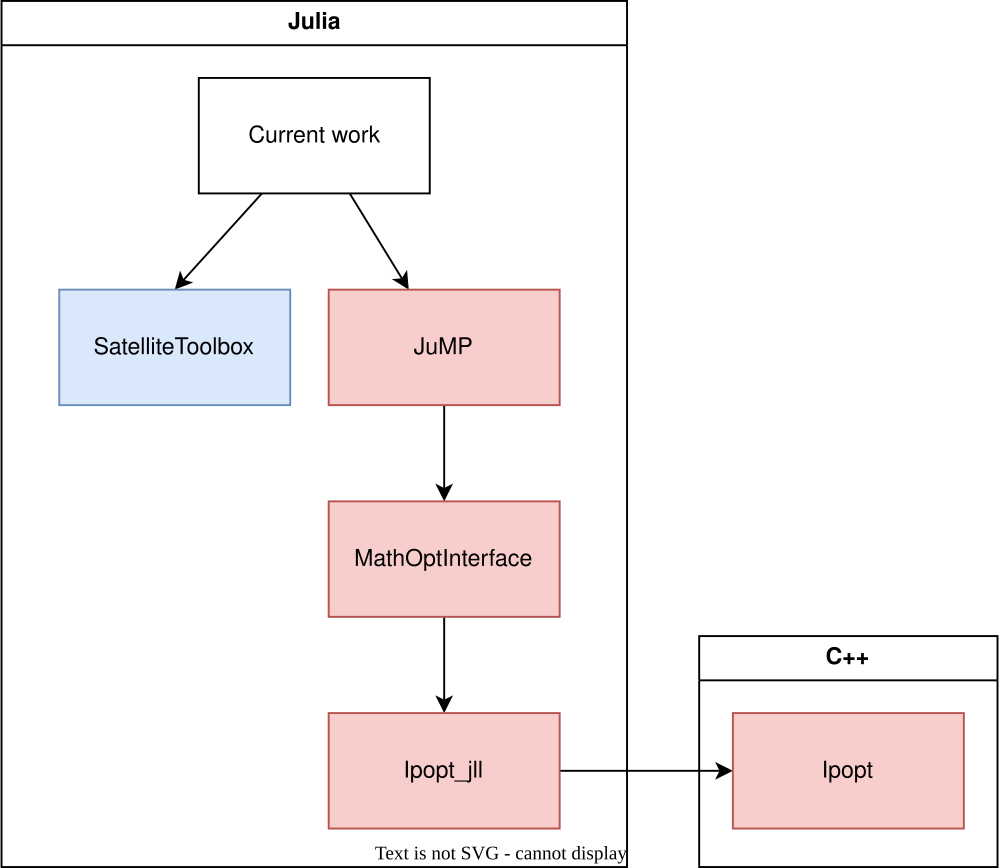
\includegraphics[width=\textwidth]{img/techstack.png}
    \caption{Relationship of code components}
    \label{fig:tech_stack}
\end{figure}

\section{Lambert problem formulations}

\section{Optimal impulsive maneuver problem statement} \label{sec:impulsive_statement}

algo usado